\documentclass[./FinalReport.tex]{subfiles}

\begin{document} %implementation
\subsection{Building Geometry in Blender}
The surfaces used for analysis are built in the 3D modeling system Blender. Blender provides simple tools for creating and editing NURBS surfaces, such as the cylinder in FIgure \ref{fig:cylinder} or the surface bump in Figure \ref{fig:bump}. Blender provides  a rather robust scripting feature where python scripts can be utilized to manipulate the 3D scene. The custom blender script \code{BlenderExportNURBS.py} (found in \code{Shoreline/Scripts/}) was written to export NURBS geometry from Blender into a simple format which can be read into the application code. 
\begin{figure}[!htbp]
  \centerline{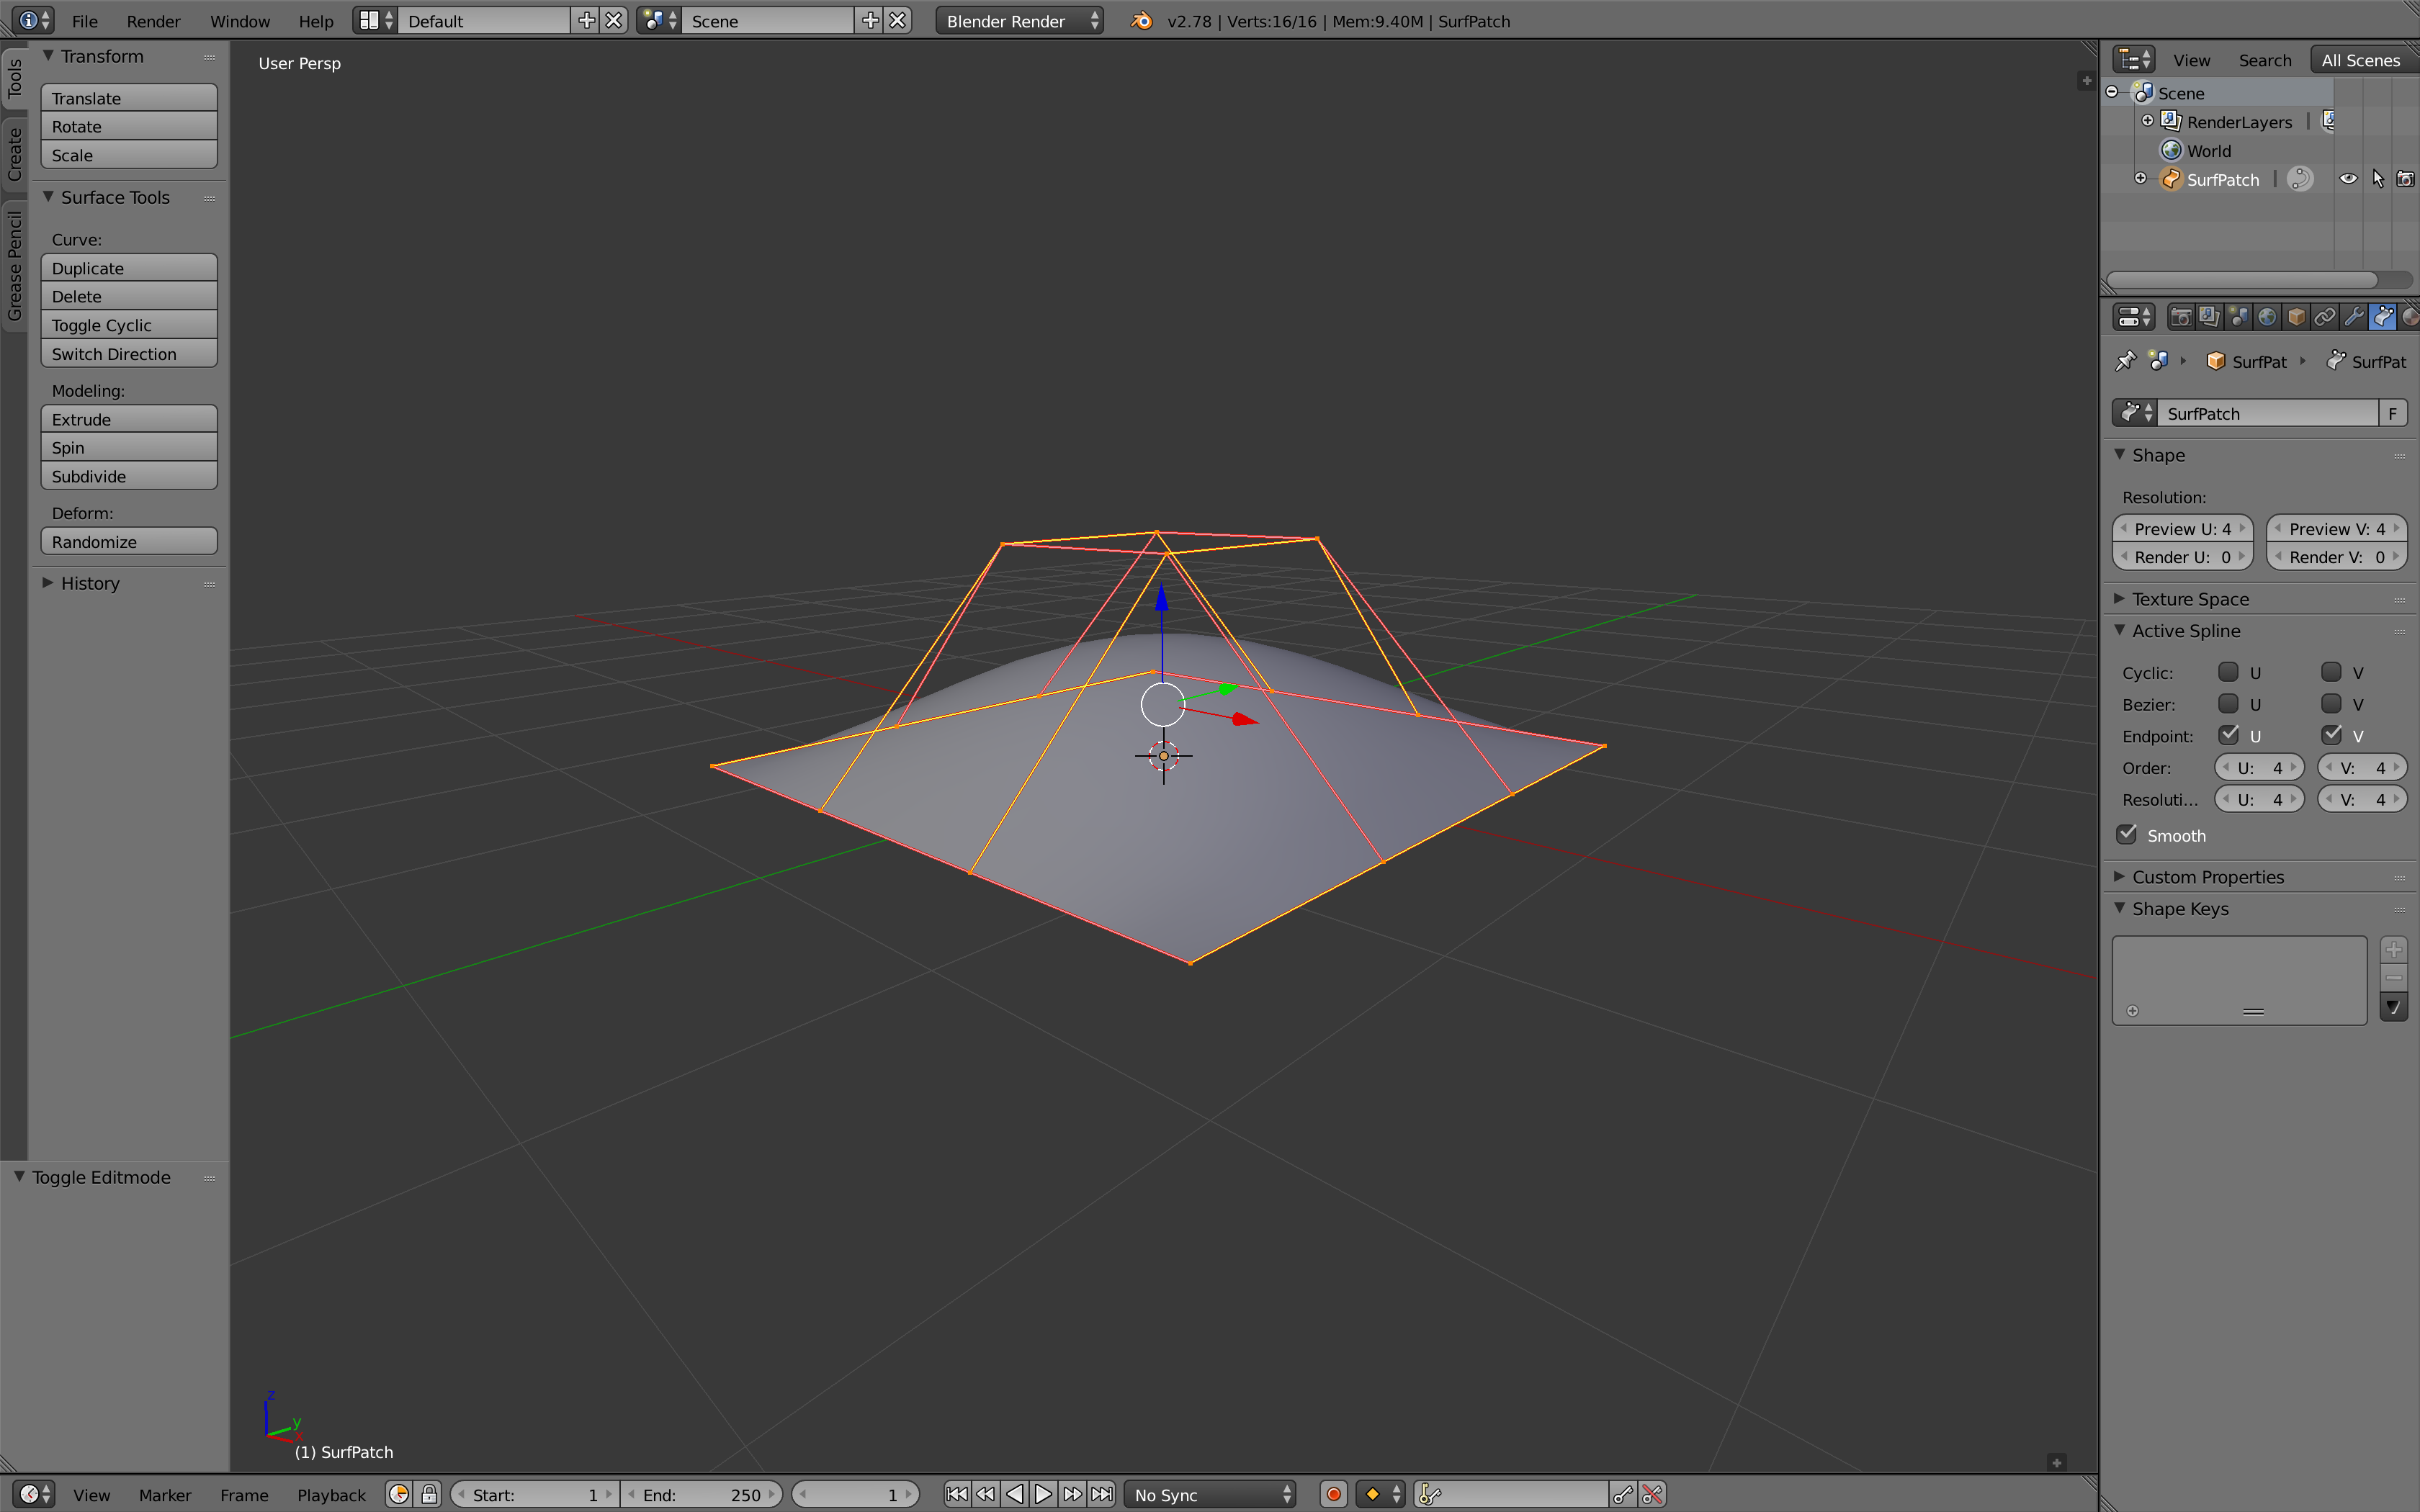
\includegraphics[width=4in]{./figures/SrfBumpBlender}}
  \caption{NURBS surface bump created in Blender}
  \label{fig:bump}
\end{figure}

\subsection{Surface Class}
The \code{Surface} class is responsible for storing information about the imported surface, and prepares it for analysis. A \code{Surface} object is initialized with the file path of a surface exported from Blender. This file is read in with \code{import\_Geometry(string geomFile)} which parses the polynomial order, the number of basis functions and the list of control points from this file. Knot vectors are not stored directly in Blender, but are computed, so the process for building knot vectors in Blender has been adapted for this application code within the \code{compute\_knots()} set of functions. Generally, Blender will export single element geometries, which is generally not suitable for analysis. As such, a surface refinement tool can be run on the surface \code{refine()} which performs knot insertion, doubling the number of knot spans in each direction. The \code{Surface} object is made analysis ready with the command \code{ready\_analysis()}, which builds the IEN array and computes the extraction operator along with the extracted control points (control points defining each element individually). The IEN array is built via a call to \code{ien\_2D()} which calls \code{ien\_1D(int uv)} for each direction, and then tensor products together the output of those calls. The extraction operator is similarly built via a call to \code{extraction\_2D()} which calls \code{extraction\_1D(int uv)} in each direction and tensor products together the output of each element's 1D extraction operator in the $u$ and $v$ directions. 

\subsection{Problem Class}
The \code{Problem} class is responsible for building boundary conditions and forcing functions for analysis over the imported surface. Its constructor \code{Problem(Surface *srf, string problemType)} takes in a pointer to the \code{Surface} object, along with a string denoting the problem to be solved. That string is compared to the tags on each of the implemented problems. The \code{Problem} object then computes a vector of booleans \code{BC} which indicates which basis function is associated with a boundary condition. A corresponding vector of doubles \code{g} is computed which stores the value of the boundary conditions. Similarly, a vector of doubles \code{forcing} is computed which returns the value of the forcing function. We will keep the forcing to zero for now, but this will become useful moving forward. 

\subsection{Solver Class}
The final component of the application code is the \code{Solver} class. A \code{Solver} object is created with the constructor \code{Solver\_LaplaceBeltrami(Surface *srf, Problem *prb)}, taking in a pointer to a \code{Surface} and a \code{Problem} object. The \code{Solver} object is responsible for managing all of the PETSc data structures, and builds and solves the numerical solution to the problem at hand. It is also responsible for printing the solution and various data structures to files which can be read into and analyzed or visualized in MATLAB. 

PETSc objects are built with the method \code{petsc\_setup()}, which allocates the tangent matrix \code{Tangent}, the right hand side vector \code{rhs} and the solution vector \code{sol\_vec}. The sparsity of the tangent matrix is determined by the number of degrees of freedom within elements on the surface. the solver uses the \code{KSPGMRES} solver with a \code{PCLU} preconditioner in order to do an exact solution to the matrix system in one iteration. 

The other important class methods in the \code{Solver} class are \code{element\_formation(int e)} and \code{element\_assembly()}. The formation routine forms the local element stiffness matrix and right hand side over element \code{e}. This is done with a loop over quadrature points nested with a loop over basis functions defined over the element. The assembly step loops over each element, calling \code{element\_formation()} and assembles those into the global system matrix. This process is nearly identical to typical element formation and assembly steps found in classical finite element methods. 

\end{document}